\begin{center}
  \textbf{Отчёт лабораторной работы №\envReportLabNumber}
\end{center}

\textbf{Тема}:
<<\envReportTitle>>

\textbf{Цель}: ...

\begin{center}
  \textbf{1-ая часть лабораторной работы}
\end{center}

Беру методичку с сайта \url{http://sinpix.ru} по теме <<Матричные игры>> \cite{MethodSinpixMatrixGames}.

\textbf{Условие}: 

Две компании, занимающиеся производством антивирусного программного обеспечения,
практически полностью делят рынок некоторого региона.
Разрабатывая новую версию программного продукта для мобильных телефонов,
каждая из компаний может использовать один из четырех вариантов продвижения нового программного продукта на рынок,
который влияет на конечную стоимость продукции.
В зависимости от сделанного выбора компании могут установить цену реализации единицы продукции на уровне 25, 22, 19 и 16 условных единиц соответственно.
Соотношение цен реализации и себестоимость представлены в таблице:

\begin{table}[h!]
  \centering

  % \scriptsize

  \caption{Данные к заданию}
  \label{tab:part1_option5}

  \begin{tabular}{|l|l|l|l|l|l|l|l|l|l|l|} 
    \hline
    
    \multirow{2}{*}{\textbf{\thead{Вариант \\продвижения\\ нового продукта}}}
    & \multirow{2}{*}{\textbf{\thead{Цена реализации\\ единицы продукции,\\ у.е.}}}
    &\multicolumn{2}{c|}{\textbf{\thead{Полная себестоимость\\единицы продукции,\\ у.е.}}} \\
    \cmidrule{3-4}&&Компания А & Компания B 
    \\\hline
    1 &25 &17           &$21 - 0,1*N$ \\ \hline
    2 &22 &15           &$10 + 0,1*N$ \\  \hline
    3 &19 &$10 + 0,1*N$ &10           \\ \hline
    4 &16 &$5 + 0,1*N$  &5            \\ \hline
  \end{tabular}
\end{table}

N - номер варианта, предложенный преподавателем.

В результате маркетингового исследования рынка была определена функция спроса на программные продукты:

$Y = 20 - 0,5 * X$

Y - количество продукции, которое будет реализовано в регионе (тыс. ед.),

X - средняя цена продукции компаний, у.е.

Значения долей продукции, реализованной компанией А, зависят от соотношения цен на продукцию компании А и компании В.
Маркетинговое исследование позволило установить эту зависимость:

\newpage

\begin{table}[h!]
  \centering

  % \scriptsize

  \caption{Данные к заданию}
  \label{tab:part1_option5}

  \begin{tabular}{|l|l|l|l|l|l|l|l|l|l|l|} 
    \hline
    \multicolumn{2}{|c|}{\textbf{\thead{Цена реализации\\ 1 ед. продукции,\\ у.е.}}}
    &\multirow{2}{*}{\textbf{\thead{Доля реализованной\\ продукции\\ компании А}}} \\
    \cmidrule{1-2} Компания A & Компания B &\\ \hline
    25  &25 &0,31 \\ \hline
    25  &22 &0,33 \\ \hline
    25  &19 &0,25 \\ \hline
    25  &16 &0,2  \\ \hline
    22  &25 &0,4  \\ \hline
    22  &22 &0,35 \\ \hline
    22  &19 &0,32 \\ \hline
    22  &16 &0,28 \\ \hline
    19  &25 &0,52 \\ \hline
    19  &22 &0,48 \\ \hline
    19  &19 &0,4  \\ \hline
    19  &16 &0,35 \\ \hline
    16  &25 &0,6  \\ \hline
    16  &22 &0,58 \\ \hline
    16  &19 &0,55 \\ \hline
    16  &16 &0,5  \\ \hline
  \end{tabular}
\end{table}

\begin{enumerate}
  \item[1.] Существует ли в данной задаче ситуация равновесия при выборе варианта продвижения продукта на рынок обоими компаниями?
  \item[2.] Существуют ли варианты, которые компании заведомо не будут выбирать вследствие невыгодности?
  \item[3.] Сколько продукции будет реализовано в ситуации равновесия?
  Какая компания получит больше прибыль в ситуации равновесия?
  Какая компания будет иметь большую долю рынка в ситуации равновесия?
  Дайте краткую экономическую интерпретацию результатов решения задачи.
\end{enumerate}

\newpage

\begin{center}
  \textbf{Ход работы}
\end{center}

Одной из главных задач каждого предприятия является максимизация прибыли от реализации продукции.
Но в данном случае более важной проблемой является конкурентная борьба.
В конкурентном конфликте выигрыш будет определяться не размером прибыли каждого предприятия, а разностью их прибылей.
При таком подходе конфликт можно рассматривать как матричную игру двух игроков с нулевой суммой, т.к. выигрыш одного предприятия равен проигрышу другого.
Формализуем конфликтную ситуацию - составим платежную матрицу.
Для этого определим стратегии каждого игрока:
\begin{enumerate}
  \item[-] А1 - предприятие А выбирает технологию 1;
  \item[-] А2 - предприятие А выбирает технологию 2;
  \item[-] А3 - предприятие А выбирает технологию 3;
  \item[-] А4 - предприятие А выбирает технологию 4;
  \item[-] В1 - предприятие В выбирает технологию 1;
  \item[-] В2 - предприятие В выбирает технологию 2;
  \item[-] В3 - предприятие В выбирает технологию 3;
  \item[-] В4 - предприятие В выбирает технологию 4.
\end{enumerate}

Средняя цена на продукцию буду считать по формуле (\ref{equ:part1_x}).

\begin{equation} \label{equ:part1_x}
  X = \frac{p_1 + p_2}{2}
\end{equation}

Функция спроса представлена формулой (\ref{equ:part1_y}).

\begin{equation} \label{equ:part1_y}
  Y = 20 - 0,5 \cdot X
\end{equation}

У предприятия A купят $d \cdot 100\%$ от всей купленной продукции по формуле (\ref{equ:part1_YD}).

\begin{equation} \label{equ:part1_YD}
  Y d
\end{equation}

У предприятия B купят $(1-d) \cdot 100\%$ от всей купленной продукции по формуле (\ref{equ:part1_Y1d}).

\begin{equation} \label{equ:part1_Y1d}
  Y (1 - d)
\end{equation}

Прибыль A считается по формуле (\ref{equ:part1_pribA}).

\begin{equation} \label{equ:part1_pribA}
  \text{Доход} \equiv \text{прибыль}A = Y d p_1 - Y d s_1
\end{equation}

Прибыль B считается по формуле (\ref{equ:part1_pribB}).

\begin{equation} \label{equ:part1_pribB}
  \text{Затраты} \equiv \text{прибыль}B = Y (1-d) p_2 - Y (1-d) s_2
\end{equation}

Элемент платежной матрицы находится по формуле (\ref{equ:part1_aij}).

\begin{equation} \label{equ:part1_aij}
  a_{ij} = \text{прибыль }A - \text{прибыль}B \equiv \text{Прибыль} = \text{Доход} - \text{Затраты}
\end{equation}

\newpage

Вычисления произведены в Google Таблицах \cite{GoogleTables}.
Google таблицы выбрал, так как там сразу можно выбрать приятные цвета для закрашивания ячеек. (В черно-белом отчете не увидеть).

Файл > Скачать > Microsoft Excel (XLSX)

Открываю файл в Libre Office \cite{LibreOffice}.

Сохраняю картинку выделенных ячеек:

U17 > Shift > A1 > File > Export > Selection > PNG - Portable Network Graphics (.png) \\
> Name > part1\_option5 > Save > OK

Результаты вычисления показаны на рис.~\ref{fig:part1_option5}.

\begin{figure}[!h]
  \centering

  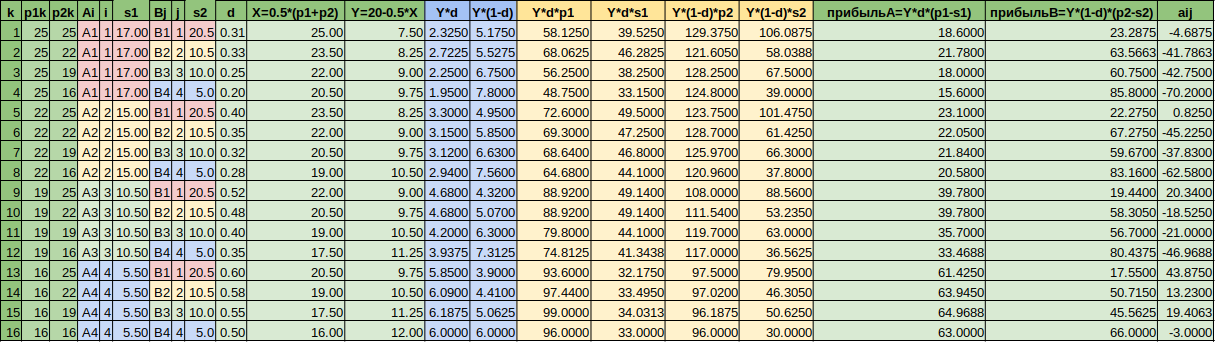
\includegraphics[width=18cm]
  {../sources/part1_option5.png}

  \caption{Расчеты элемента платежной матрицы для варианта 5}

  \label{fig:part1_option5}
\end{figure}

Сохраняю картинку выделенных ячеек:

AE6 > Shift > Z1 > File > Export > Selection > PNG - Portable Network Graphics (.png) \\
> Name > part1\_option5 > Save  > OK

Высчитанные элементы $a_{ij}$ из рис.~\ref{fig:part1_option5} перенесены в 2D-матрицу на рис.~\ref{fig:part1_option5_matrix}.
В этой матрице также найдена седловая точка.

\begin{figure}[!h]
  \centering

  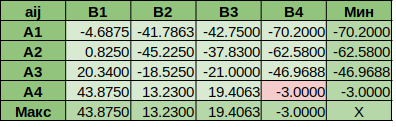
\includegraphics[width=12cm]
  {../sources/part1_option5_matrix.png}

  \caption{Платежная матрица для варианта 5}

  \label{fig:part1_option5_matrix}
\end{figure}

\subparagraph{Задание 1} \hspace{0pt}

Проверим наличие ситуации равновесия - седловой точки. Для это найдем нижнюю и верхнюю цены игры.

В каждой строчке определим минимальный элемент и запишем его в новом столбце,
а из найденных минимальных выберем максимальный:

$\alpha = max(-43,875; 13,23; 19,4063; -3) = -3$

$\alpha = -3$ - нижняя цена игры.

В каждом столбце найдем максимальный элемент и запишем их в новой строке и из них
выберем минимальный

$\beta = min(-70,2; -62,58; -46,9688; -3) = -3$

$\beta = -3$ - верхняя цена игры

Так как $\alpha = \beta = -3$, то в конфликтной ситуации есть точка равновесия - седловая
точка, которую образуют стратегии (А4, В2).

Если одно предприятие будет придерживаться своей оптимальной стратегии,
то самое лучшее поведение второго предприятия - также придерживаться своей оптимальной стратегии.
В приложении к условию это означает, что предприятиям необходимо
использовать свои четвертые технологии и минимальные цены реализации.

\textbf{Ответ}: Ситуация равновесия доступна при стратегиях (A4, B4). 

\subparagraph{Задание 2} \hspace{0pt}

Определим наличие заведомо невыгодных стратегий у предприятий.
Так как элементы четвертой строки больше соответствующих элементов первой, второй и третьей строки,
то стратегии А1, A2 и А3 - заведомо невыгодные, так как предприятие А стремится максимизировать разницу прибылей.

Аналогично для предприятия В. Все элементы четвертого столбца меньше соответствующих элементов первого, второго и третьего столбцов,
значит стратегии В1, В2, B3 - заведомо невыгодные (доминируемые).

\textbf{Ответ}: Предприятие A не будет выбирать технологии 1, 2 и 3.
Предприятие B не будет выбирать технологии 1, 2 и 3.

\subparagraph{Задание 3} \hspace{0pt}

При стратегии (A4, B4):
\begin{enumerate}
  \item[-] $X(A4, B4) = 16 \text{ д. е.}$ - средняя цена на продукцию;
  \item[-] $Y(A4, B4) = 12 \text{ тыс. ед.} = 12000 \text{ ед.}$ - результат функции спроса;
  \item[-] $Y(A4, B4) \cdot  d(A4, B4) = [12 \cdot 0,5] = 6 \text{ тыс. ед.} = 6000 \text{ ед.}$ - купят у предприятия A;
  \item[-] $Y(A4, B4) \cdot (1 - d(A4, B4)) = [12 \cdot (1-0,5)] = 6 \text{ тыс. ед.} = 6000 \text{ ед.}$ - купят у предприятия B.
\end{enumerate}

\textbf{Ответ}: В ситуации равновесия будет реализовано ($Y = 20 - 0,5 \cdot \frac{16 + 16}{2} = 12$) 12000 единиц продукции.
У первого предприятия купят 6000 ед. продукции, а у второго 6000 ед. продукции.
В выигрышном положении будет и предприятие А, и предприятие Б.

\newpage

\begin{center}
  \textbf{2-ая часть лабораторной работы}
\end{center}

Беру методичку с сайта \url{http://sinpix.ru} по теме <<Матричные игры>> \cite{MethodSinpixMatrixGames}.

\textbf{Условие}: 

Матричную игру 2х2 решить в смешанных стратегиях:

\begin{enumerate}
  \item[1)] аналитически (для игрока А); геометрически (для игрока В)
  \item[2)] провести моделирование результатов игры с помощью таблицы равномерно распределенных случайных чисел, разыграв 30 партий;
  определить относительные частоты использования чистых стратегий каждым игроком и средний выигрыш,
  сравнив результаты с полученными теоретически в п.1.
\end{enumerate}

\textbf{Вариант 5}: $ \begin{pmatrix}
  13&5\\
  7&8
\end{pmatrix} <= \begin{pmatrix}
  A_1 \cap B_1 & A_1 \cap B_2\\
  A_2 \cap B_1 & A_2 \cap B_2
\end{pmatrix}$

\begin{center}
  \textbf{Ход работы}
\end{center}

\subparagraph{Задание 1} \hspace{0pt}

Найдем аналитически оптимальную стратегию игрока А и соответствующую цену игры $X^*(p_1, p_2)$, $ v $.

Так как $X^*$ - оптимальная, то она должна гарантировать средний выигрыш игроку A, равный цене игры при любом поведении игрока B:

\begin{enumerate}
  \item[-] для стратегии В1: $13 p_1 + 7 p_2 = v$;
  \item[-] для стратегии В2: $5 p_1 + 8 p_2 = v$.
\end{enumerate}

С учетом того, что сумма компонентов смешанной стратегии равна 1, получаем систему уравнений: $
\begin{cases}
  13 p_1 + 7 p_2 = v \\
  5 p_1 + 8 p_2 = v \\
  p_1 + p_2 = 1
\end{cases}
$

Вычтем из первого уравнения второе: $-
\begin{cases}
  13 p_1 + 7 p_2 = v \\
  5 p_1 + 8 p_2 = v \\
\end{cases}
$

$13 p_1 - 5 p_1 + 7 p_2 - 8 p_2 = v - v$

$8 p_1 - 1 p_2 = 0$

$p_2 = 8 p_1$

Значит: $
\begin{cases}
  13 p_1 + 7 p_2 = v \\
  5 p_1 + 8 p_2 = v \\
  p_1 + p_2 = 1 \\
  p_2 = 8 p_1
\end{cases} =>
\begin{cases}
  13 p_1 + 7 p_2 = v \\
  5 p_1 + 8 p_2 = v \\
  p_1 + 8 p_1 = 1 \\
  p_2 = 8 p_1
\end{cases} =>
\begin{cases}
  13 p_1 + 7 p_2 = v \\
  5 p_1 + 8 p_2 = v \\
  9 p_1 = 1 \\
  p_2 = 8 p_1
\end{cases}
$

$ =>
\begin{cases}
  13 p_1 + 7 p_2 = v \\
  v = 5 p_1 + 8 p_2 \\
  p_1 = \frac{1}{9} \\
  p_2 = \frac{8}{9}
\end{cases} =>
\begin{cases}
  13 p_1 + 7 p_2 = v \\
  v = \frac{5}{9} + \frac{64}{9} \\
  p_1 = \frac{1}{9} \\
  p_2 = \frac{8}{9}
\end{cases} =>
\begin{cases}
  13 p_1 + 7 p_2 = v \\
  v = \frac{69}{9} = \frac{23}{3} \\
  p_1 = \frac{1}{9} \\
  p_2 = \frac{8}{9}
\end{cases} =>
\begin{cases}
  v = \frac{23}{3} \\
  p_1 = \frac{1}{9} \\
  p_2 = \frac{8}{9}
\end{cases}
$

Итак: $X^*(p_1, p_2) = X^*(\frac{1}{9}, \frac{8}{9})$, $v=\frac{23}{3}$.

Найдем геометрически оптимальную смешанную стратегию игрока В: $Y^*(q_1, q_2)$.

Стратегию $A_1$ изобразим точками с ординатами 13 и 5 на прямых $B_1$ и $B_2$ соответственно.
Стратегию $A_2$ - точками с ординатами 7 и 8 (см. рис. 1).

$\begin{pmatrix}
  13&5\\
  7&7
\end{pmatrix} =>
\begin{pmatrix}
  A_1(0; 13)  &A_2(1; 5)\\
  A_1(0; 7)   &A_2(1; 7)
\end{pmatrix} <=
\begin{pmatrix}
  a_{11}      &a_{21}\\
  a_{12}      &a_{22}
\end{pmatrix}$

\begin{figure}[!h]
  \centering

  \includegraphics[width=12cm]
  {assets/export/part2-option5-Page-1.pdf}

  \caption{Платежная матрица для варианта 5}

  \label{fig:part1_option5_matrix}
\end{figure}

Каждой точке на отрезке [0; 1] соответствует смешанная стратегия игрока В.
Среди них оптимальной будет та, которая определяется самой низкой точкой ломанной А1МА2, т.е. точкой М.
Для нахождения компонентов оптимальной стратегии игрока В надо найти координаты точки М,
причем если $M(x, y)$, то $q_1 = 1 - x$, $q_2 = x$, $v = y$.
Для этого найдем уравнения прямых А1А1 и А2А2, воспользовавшись уравнением прямой, проходящей через две точки:
$\frac{x-x_1}{x_2 - x_1} = \frac{y-y_1}{y_2 - y_1}$.

Так как $A_1(x_1, y_1) = A_1(0; 13)$ и $A_1(x_2, y_2) = A_1(1; 5)$, то $\begin{cases}
  x_1 = 0 \\
  x_2 = 1 \\
  y_1 = 13 \\
  y_2 = 5
\end{cases} => \frac{x-0}{1 - 0} = \frac{y-13}{5 - 13} => \\
=> x = \frac{y-13}{-8} => -8 x = y - 13 => 8x + y - 13 = 0$

Т. е. уравнение прямой А1А1 имеет вид: $8x + y - 13 = 0$.

Так как $A_2(x_1, y_1) = A_2(0; 7)$ и $A_2(x_2, y_2) = A_2(1; 8)$, то $\begin{cases}
  x_1 = 0 \\
  x_2 = 1 \\
  y_1 = 7 \\
  y_2 = 8
\end{cases} => \frac{x-0}{1 - 0} = \frac{y-7}{8 - 7} => \\
=> x = y-7 => x - y + 7 = 0$

Т. е. уравнение прямой А2А2 имеет вид: $x - y + 7 = 0$.

Найдем координаты точки М, решив систему уравнений прямых А1А1 и А2А2:

$\begin{cases}
  8x + y - 13 = 0 \\
  x - y + 7 = 0
\end{cases} => +\begin{cases}
  8x + y - 13 = 0 \\
  x - y + 7 = 0
\end{cases} => \begin{cases}
  8x + x + y - y - 13 + 7 = 0 + 0 \\
  x - y + 7 = 0
\end{cases} =>$

$=> \begin{cases}
  9x -6 = 0
  y = x + 7
\end{cases} => +\begin{cases}
  x = \frac{6}{9} = \frac{2}{3} \\
  y = \frac{2}{3} + \frac{7 * 3}{3}
\end{cases} => \begin{cases}
  x = \frac{2}{3} \\
  y = \frac{23}{3}
\end{cases} => M(x, y) = M(\frac{2}{3}, \frac{23}{3})$

$\begin{cases}
  M(x; y) = M(\frac{2}{3}, \frac{23}{3})\\
  y = v
\end{cases} => v = \frac{23}{3} = 7,(6)$

$\begin{cases}
  q_1 = 1 - x \\
  q_2 = x
\end{cases} => +\begin{cases}
  q_1 = \frac{1 * 3}{3} - \frac{2}{3} \\
  q_2 = \frac{2}{3}
\end{cases} => \begin{cases}
  q_1 = \frac{1}{3} \\
  q_2 = \frac{2}{3}
\end{cases} => Y^*(q_1, q_2) = Y^*(\frac{1}{3}, \frac{2}{3})$

\textbf{Ответ}: 
\begin{enumerate}
  \item[-] $X^*(\frac{1}{9}; \frac{8}{9}) = X^*(0,(1); 0,(8))$;
  \item[-] $v = \frac{23}{3} = 7,(6)$;
  \item[-] $Y^*(\frac{1}{3}; \frac{2}{3}) = Y^*(0,(3); 0,(6))$.
\end{enumerate}

\subparagraph{Задание 2} \hspace{0pt}

Проведем моделирование результатов решения с помощью таблицы равномерно распределенных случайных чисел.
Для 30 партий хватит 60 чисел, на основе которых будут выбираться стратегии игроками.
Используемые случайные числа сгенерированы в Google Таблицах \cite{GoogleTables} функцией =СЛЧИС().
В приложении достаточно много чисел, но использовать для моделирования можно любые 60, выбранные произвольно с любого места таблицы.
Мы возьмем числа из первого блока (для игрока А используется 1, 3 и 5 столбики).

Будем выбирать стратегии игроков, используя геометрическое определение вероятности.
Так как все случайные числа из отрезка [0; 1], то чтобы стратегия А1 появлялась,
будем ее выбирать, если случайное число меньше $p_1 = \frac{1}{9} = 0,(1)$;
в остальных случаях выбирается стратегия А2.
Аналогично для игрока В.
Стратегию В1 будем выбирать, если соответствующее случайное число меньше $q_1 = \frac{1}{3} = 0,(3)$, в противном случае выбираем стратегию В1.

Заполним расчетную таблицу. Результат на рис.~\ref{fig:part2_option5}.

Файл > Скачать > Microsoft Excel (XLSX)

Открываю файл в Libre Office \cite{LibreOffice}.

Сохраняю картинку выделенных ячеек:

Q33 > Shift > A1 > File > Export > Selection > PNG - Portable Network Graphics (.png) \\
> Name > part2\_option5 > Save > OK

\begin{figure}[!h]
  \centering

  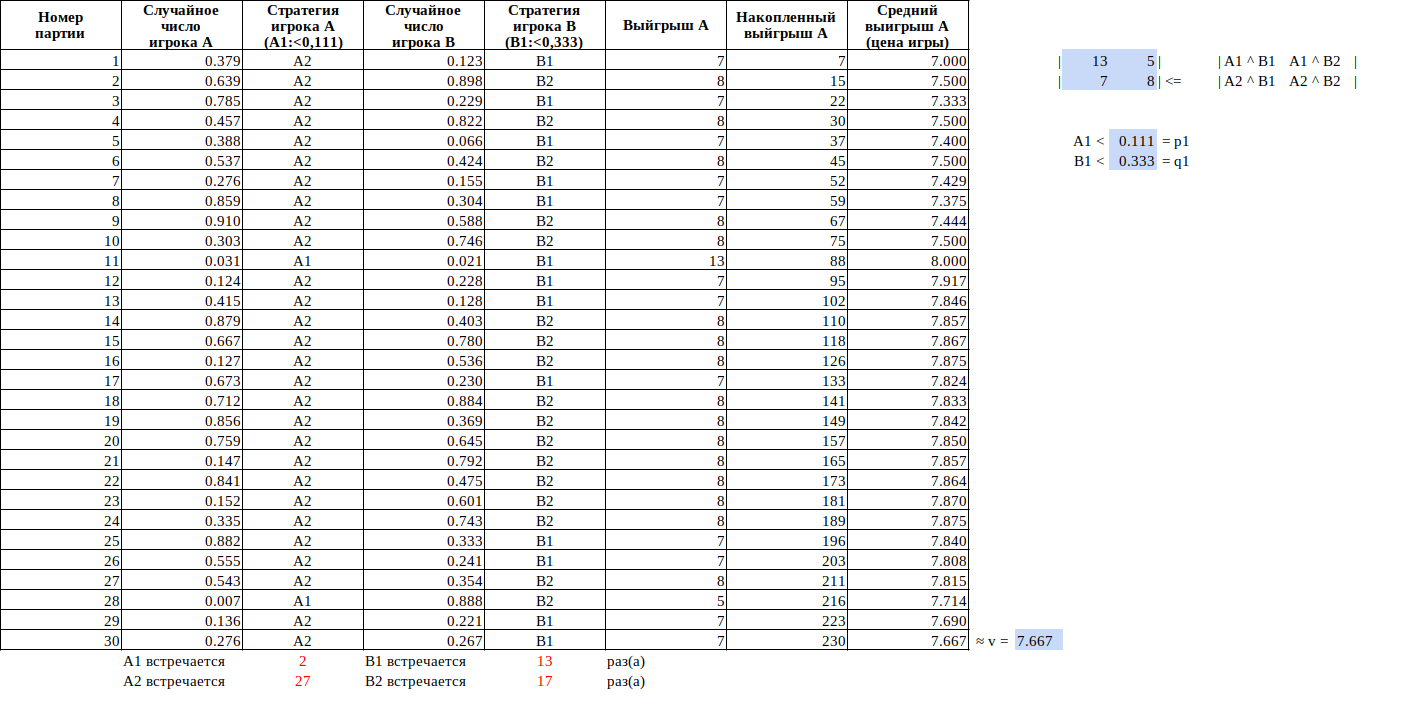
\includegraphics[width=18cm]
  {../sources/part2_option5.png}

  \caption{Расчетная таблица}

  \label{fig:part2_option5}
\end{figure}

Таким образом, в результате моделирования в 30 партиях цена игры (средний выигрыш) равен $7,7$.


Десять раз сгенерировал данные и нашел среднюю v: $\text{сред.}v = \frac{\sum^n_{i=1}}{n}$.

$\text{сред.}v = \frac{7.967+7.5+7.833+7.367+7.433+7.767+7.633+7.833+7.8+7.867}{10} = 7.7$

Этот результат согласуется с теоретической ценой игры $v = \frac{23}{3} = 7,(6) \approx 7,7$.

Частоты использования игроками своих чистых стратегий соответственно равны:
$Х(\frac{2}{30}; \frac{27}{30})$, $Y(\frac{9}{30}; \frac{20}{30})$ или
$Х(0,0(6); 0,9)$, $Y(0,3; 0,(6))$.

Сравнивая с теоретическими оптимальными стратегиями $X^*(0,(1); 0,(8))$ и $Y^*(0,(3); 0,(6))$ можно сделать вывод,
что результаты моделирования достаточно близко им соответствуют даже для небольшого количества партий.
